% % % % % % % % % % % % % % % % % % % % % % % % % % % % % % % % % % % % % % % % % % % %
%                                                                                     %
% Short Sectioned Assignment LaTeX Template Version 1.0 (5/5/12)                      %
% This template has been downloaded from: http://www.LaTeXTemplates.com               %
%                                                                                     %
% Original author:  Frits Wenneker (http://www.howtotex.com)                          %
%                                                                                     %
% Modified by: Fco Javier Sueza Rodríguez (fcosueza@disroot.org)                      %
%                                                                                     %
% Changes:                                                                            %
%	    - Custom Chapters, Sections and Subsections (titlesec package)                %
%           - Document type scrbook (oneside)                                         %
%           - Use babel-lang-spanish package and marvosym                             %
%           - Use hyperref, enumitem, tcolorbox and glossaries packages               %
%           - Use Time New Roman (mathptmx), Helvetic and Courier fonts               %
%                                                                                     %
% License: CC BY-NC-SA 3.0 (http://creativecommons.org/licenses/by-nc-sa/3.0/)        %
%                                                                                     %
% % % % % % % % % % % % % % % % % % % % % % % % % % % % % % % % % % % % % % % % % % % %

%-----------------------------------------------%
%	              Packages                  %
%-----------------------------------------------%

\documentclass[paper=a4, fontsize=11pt, oneside]{scrbook}

% ---- Text Input/Output ----- %

\usepackage[T1]{fontenc}
\usepackage[utf8]{inputenc}
\usepackage{mathptmx}
\usepackage[scaled=.92]{helvet}
\usepackage{courier}
\usepackage[indent=12pt]{parskip}

\usepackage{geometry}
\geometry{verbose,tmargin=3cm,bmargin=3cm,lmargin=2.6cm,rmargin=2.6cm}

% ---- Language ----- %

\usepackage[spanish]{babel}
\usepackage{marvosym}

% ---- Another packages ---- %

\usepackage{amsmath,amsfonts,amsthm}
\usepackage{graphics,graphicx}
\usepackage{titlesec}
\usepackage{fancyhdr}
\usepackage{tcolorbox}
\usepackage{hyperref}
\usepackage{enumitem}
\usepackage[automake]{glossaries}

%--------------------------------------------------------------------%
%                      Customizing Document                          %
%--------------------------------------------------------------------%


% ----------- Custom Chapters, Sections and Subsections -------------- %

\titleformat{\chapter}[display]
			{\bfseries\Huge}
			{Tema \ \thechapter} {0.5ex}
			{\vspace{1ex}\centering}

\titleformat{\section}[hang]
			{\bfseries\Large}
			{\thesection}{0.5em}{}

\titleformat{\subsection}[hang]
			{\bfseries\large}
			{\thesubsection}{0.5em}{}

\titleformat{\subsubsection}[hang]
			{\bfseries\large}
			{\thesubsubsection}{0.5em}{}

\hypersetup{
    colorlinks=true,
    linkcolor=black,
    urlcolor=magenta
}

% ------------------- Custom heaaders and footers ------------------- %

\pagestyle{fancyplain}

\fancyhead[]{}
\fancyfoot[L]{}
\fancyfoot[C]{}
\fancyfoot[R]{\thepage}

\renewcommand{\headrulewidth}{0pt} % Remove header underlines
\renewcommand{\footrulewidth}{0pt} % Remove footer underlines

\setlength{\headheight}{13.6pt} % Customize the height of the header

% --------- Numbering equations, figures and tables ----------------- %

\numberwithin{equation}{section} % Number equations within sections
\numberwithin{figure}{section} % Number figures within sections
\numberwithin{table}{section} % Number tables within sections

% ------------------------ New Commands ----------------------------- %

\newcommand{\horrule}[1]{\rule{\linewidth}{#1}} % Create horizontal rule command


%----------------------------------------------------------------------------------------
%	TÍTULO Y DATOS DEL ALUMNO
%----------------------------------------------------------------------------------------

\title{
\vspace{10ex}
\normalfont \normalsize
\Huge \textbf{Tarea 3: Aplicación de los Lenguajes de Marcas a la Sindicación de Contenidos}
}
\author{Francisco Javier Sueza Rodríguez}
\date{\normalsize\today}

%----------------------------------------------------------------------------------------
%                                     DOCUMENTO
%----------------------------------------------------------------------------------------
\begin{document}

\maketitle

\thispagestyle{empty}

\vspace{62ex}

\begin{center}
    \begin{tabular}{l l}
        \textbf{Centro}: & IES Aguadulce \\
        \textbf{Ciclo Formativo}: & Desarrollo Aplicaciones Web (Distancia)\\
        \textbf{Asignatura}: & Lenguajes de Marcas y Sistemas de Gestión de la Información\\
        \textbf{Tema}: & Tema 3 -  Aplicación de los Lenguajes de Marcas a la Sindicación de Contenidos\\
    \end{tabular}
\end{center}

\newpage

\tableofcontents

\newpage

\listoffigures

\newpage

\section{Caso Práctico}
Gracias al gran trabajo realizado por nuestra empresa, \textbf{PUMM Technologies}, se nos ha encargado que ampliemos nuestro ámbito de actuación ofreciendo servicios de sindicación de contenidos.

Seguiremos demostrando nuestro saber hacer y nuestros conocimientos en RSS y ATOM. Además vamos a realizar suscripciones a dichos canales utilizando el agregador de noticias Thunderbird. El programa Mozilla Thunderbird es una aplicación de gestión de correo electrónico que, además, nos permite la suscripción a canales RSS y Atom.

Vamos a utilizar el programa Mozilla Thunderbird para agregar canales de contenidos RSS o Atom relacionados con alguna empresa de mensajería/reparto para ver su funcionamiento.

\section{Enunciado}
Realiza un documento de texto (de Writer o similar, convertirlo a PDF y entregar el PDF) donde documentes la realización de cada uno de los apartados siguientes. Este documento es obligatorio, no se pasará a corregir el resto de la tarea si no se entrega este documento. En dicho documento deberás adjuntar capturas de pantalla, las explicaciones textuales de los distintos pasos necesarios que has dado y las decisiones que has tomado para conseguir realizar los apartados siguientes.

\subsection{Apartado A: RSS}
Crear un canal mediante el estándar RSS 2.0. El canal, además de los elementos obligatorios, tendrá los siguientes: El idioma utilizado (español), el correo del editor (vuestro email), la fecha de publicación y las siguientes categorías: 'paquetería', 'envíos' 'transporte urgente'.

Además tendrá las siguientes entradas:

\begin{itemize}
    \item Entrada sobre una empresa de paquetería que tú elijas con los siguientes elementos:
    \begin{itemize}
        \item Título
        \item Categoría: paquetería
        \item Fecha
        \item Contenido
        \item Enlace
    \end{itemize}

    \item Entrada sobre \href{https://logistica.cdecomunicacion.es/noticias/sectoriales/45956/aliexpress-llegada-iva-paqueteria-internacional}{cómo afectará la llegada del IVA a la paquetería internacional}. Del enlace de esta noticia se extraerán,  además de los elementos obligatorios, los siguientes: el título, la descripción, la \href{https://logistica.cdecomunicacion.es/wp-content/webp-express/webp-images/uploads/2022/12/1624960313-paquetera-iva-aduanas-1-1140x594.jpg.webp}{imagen} y la fecha de publicación.

    \item Entrada sobre los \href{https://logistica.cdecomunicacion.es/wp-content/webp-express/webp-images/uploads/2022/12/1624960313-paquetera-iva-aduanas-1-1140x594.jpg.webp}{problemas en la distribución de la paquetería internacional}. Del enlace de esta noticia se extraerán, además de los elementos obligatorios, los siguientes: el título, el link, la descripción, la \href{https://cdn0.celebritax.com/sites/default/files/styles/watermark_100/public/1642440970-denuncian-atraso-siete-meses-distribucion-paqueteria-internacional-cuba.jpg}{imagen} y la fecha de publicación.
\end{itemize}

La información de las entradas deben ser sobre los datos reales de páginas activas.

Valida el fichero RSS creado usando el servicio disponible en la web \href{https://validator.w3.org/feed/#validate_by_input}{W3C Feed Validation Service}, introduciendo el código del fichero RSS. Realiza una captura de pantalla, a página completa, de la validación que permitan mostrar que se ha realizado correctamente. Debe verse todo el navegador, no recortar la imagen. Es normal que en la validación aparezcan avisos 'warning'. Estas capturas se incluirán en el documento de texto que debes realizar. Incluye esta captura, con su correspondiente explicación textual, en el documento que debes realizar.

\subsection{Aparado B: Atom}
Crear un canal usando el estándar Atom 1.0 con los mismos datos, para el canal y las entradas, utilizados en el apartado A. En este estándar se deberán rellenar todos los elementos obligatorios, todos los elementos recomendados y todos los datos indicados explícitamente en el enunciado del apartado A.

Valida dicho fichero usando el servicio disponible en la web \href{https://validator.w3.org/feed/#validate_by_input}{W3C Feed Validation Service}. Realiza una captura de pantalla, a página completa, de la validación que permitan mostrar que se ha realizado correctamente. Debe verse todo el navegador, no recortar la imagen. Es normal que en la validación aparezcan avisos 'warning'. Estas capturas se incluirán en el documento de texto que debes realizar. Incluye esta captura, con su correspondiente explicación textual, en el documento que debes realizar.

\subsection{Aparatado C: Inclusión del Canal de Noticias en la Página Web}
Modifica la web que has realizado en la tarea 2 incluyendo una carpeta llamada feed que contenga los dos archivos de las actividades A y B (canal.rss y canal.atom). En caso de no haber entregado la tarea 2 se debe utilizar uno de los dos ejemplos que se proporcionaban en dicha tarea 2 como base para crear la funcionalidad el menú.

Añade todo lo necesario para que en el pie de la página web principal tenga dos imágenes (logotipos rss y atom) con enlaces a los canales de noticias. Incluye todo lo necesarios para su funcionamiento.

\subsection{Aparado D: Utilización de Agregador de Contenido}
Descarga e instala el programa de la web oficial \url{https://www.thunderbird.net/es-ES/}, y  agrega un canal de noticias de una empresa de mensajería que escojas. Realiza capturas de todo el proceso, teniendo en cuenta que, en todas las capturas deberá aparecer tu perfil de Moodle. Añade las capturas y las explicaciones de dichas capturas al documento PDF.

Debes buscar dentro de la web de la empresa elegida un archivo de este \href{https://e00-marca.uecdn.es/rss/portada.xml}{estilo}, en este caso es el canal rss de la web deportiva "marca".

\section{Soluciónes}
En esta tarea vamos a trabajar con canales de noticias tanto RSS como Atom, incluyéndolos, además, en la página web creada en el Tema 2 y usando un agregador de feeds, en nuestro caso Thunderbird, para agregar un canal de noticias.

\subsection{Solución Apartado A: RSS}

En primer lugar hemos creado un canal RSS con toda la información que se nos pide y con 3 secciones. El fichero RSS se incluye dentro del archivo comprimo de esta práctica, aunque en la siguiente figura podemos ver una captura de su validación en el validador de la W3C.

\begin{figure}[H]
    \centering
    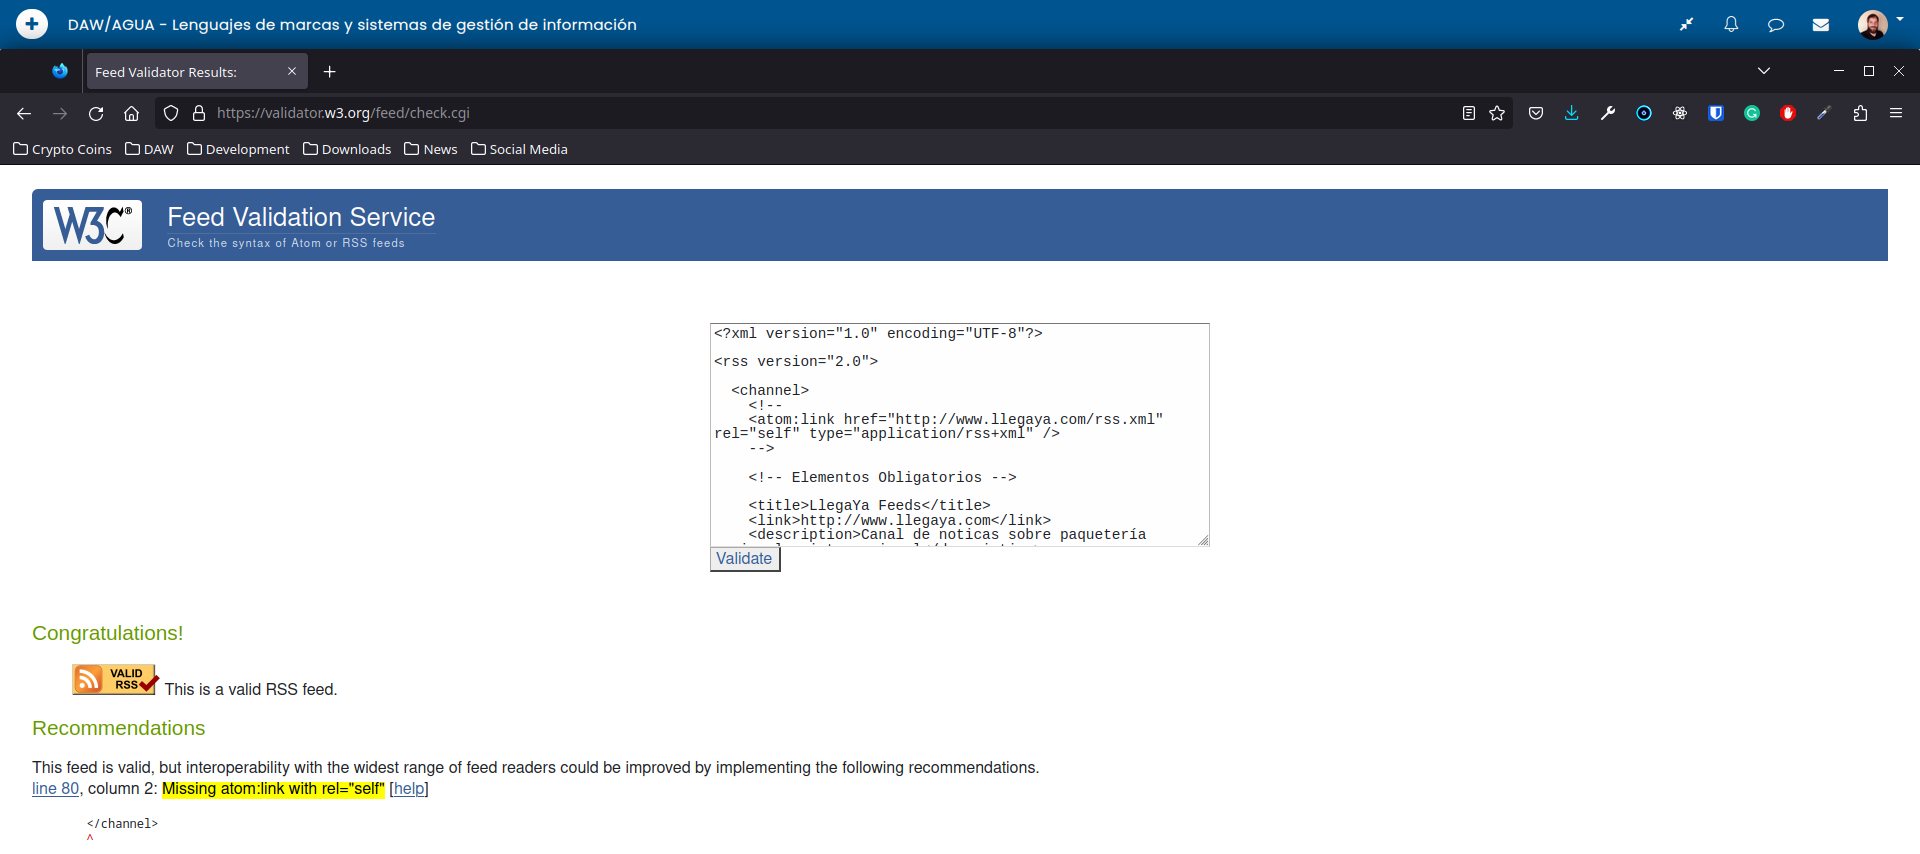
\includegraphics[scale=0.30]{rss-validation.png}
    \caption{Validación del canal RSS}
\end{figure}

Como apunte decir que aunque el fichero valida correctamente, pero se nos hace una recomendación y es que incluyamos un par de líneas para mantener la compatibilidad con atom, aunque nosotros vamos a dejar el fichero como está.

\subsection{Solución Apartado B: Atom}
Al igual que en la sección anterior, hemos creado el fichero canal.atom con el canal de noticias codificado con el estándar Atom. En la siguiente imagen podemos ver la validación de dicho fichero en el validador de la W3C.

\begin{figure}[H]
    \centering
    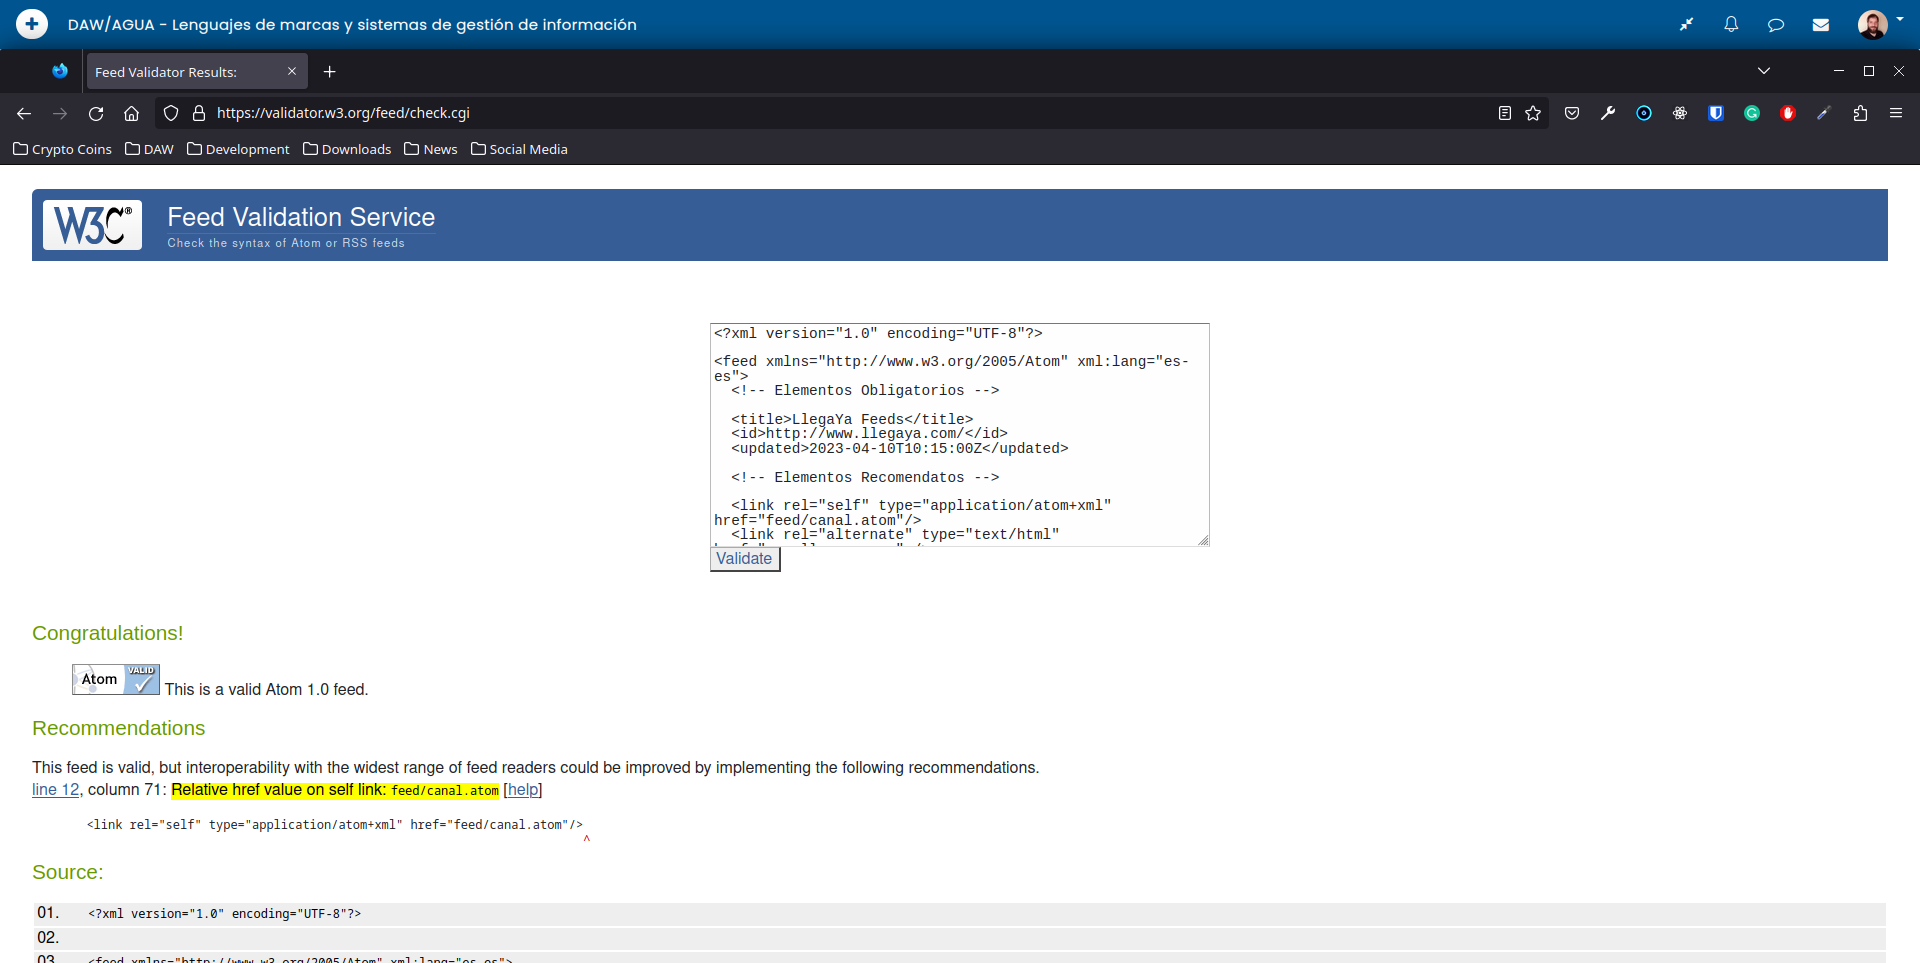
\includegraphics[scale=0.30]{atom-validation.png}
    \caption{Validación de canal Atom}
\end{figure}

Al igual que con el fichero RSS, este fichero se valida correctamente, aunque también nos hace una sugerencia, la cual es incluir el URI absoluto del canal Atom en los enlaces con el atributo rel="self", aunque ya que nuestro canal no esta colgado en la red esto es complicado, por lo que se ha dejado la ruta absoluta.

\subsection{Solución Apartado C: Añadiendo los canales a la Web}
En este punto, vamos a incluir los canales en la página web que creamos en la tarea del tema 2. En primer lugar, hemos creado una carpeta llamada \textbf{feed} donde hemos incluido los ficheros de los dos canales. A continuación, hemos descargado las \textbf{imágenes} y los enlaces que nos ha generado el validador de la W3C para cada uno de los archivos.

Una vez con todos los archivos en sus carpetas correspondientes hemos procedido a \textbf{añadir los dos canales a la página web}, en concreto en el pie de página, donde aparecerán dos iconos con los logos tanto de RSS como de Atom donde los usuarios podrán pulsar para descargar los canales de noticias. También se ha añadido una clase CSS para darles un poco de estilo.

En la siguiente captura, se puede ver la página principal con los dos iconos de los canales añadidos en el pie de página.

\begin{figure}[H]
    \centering
    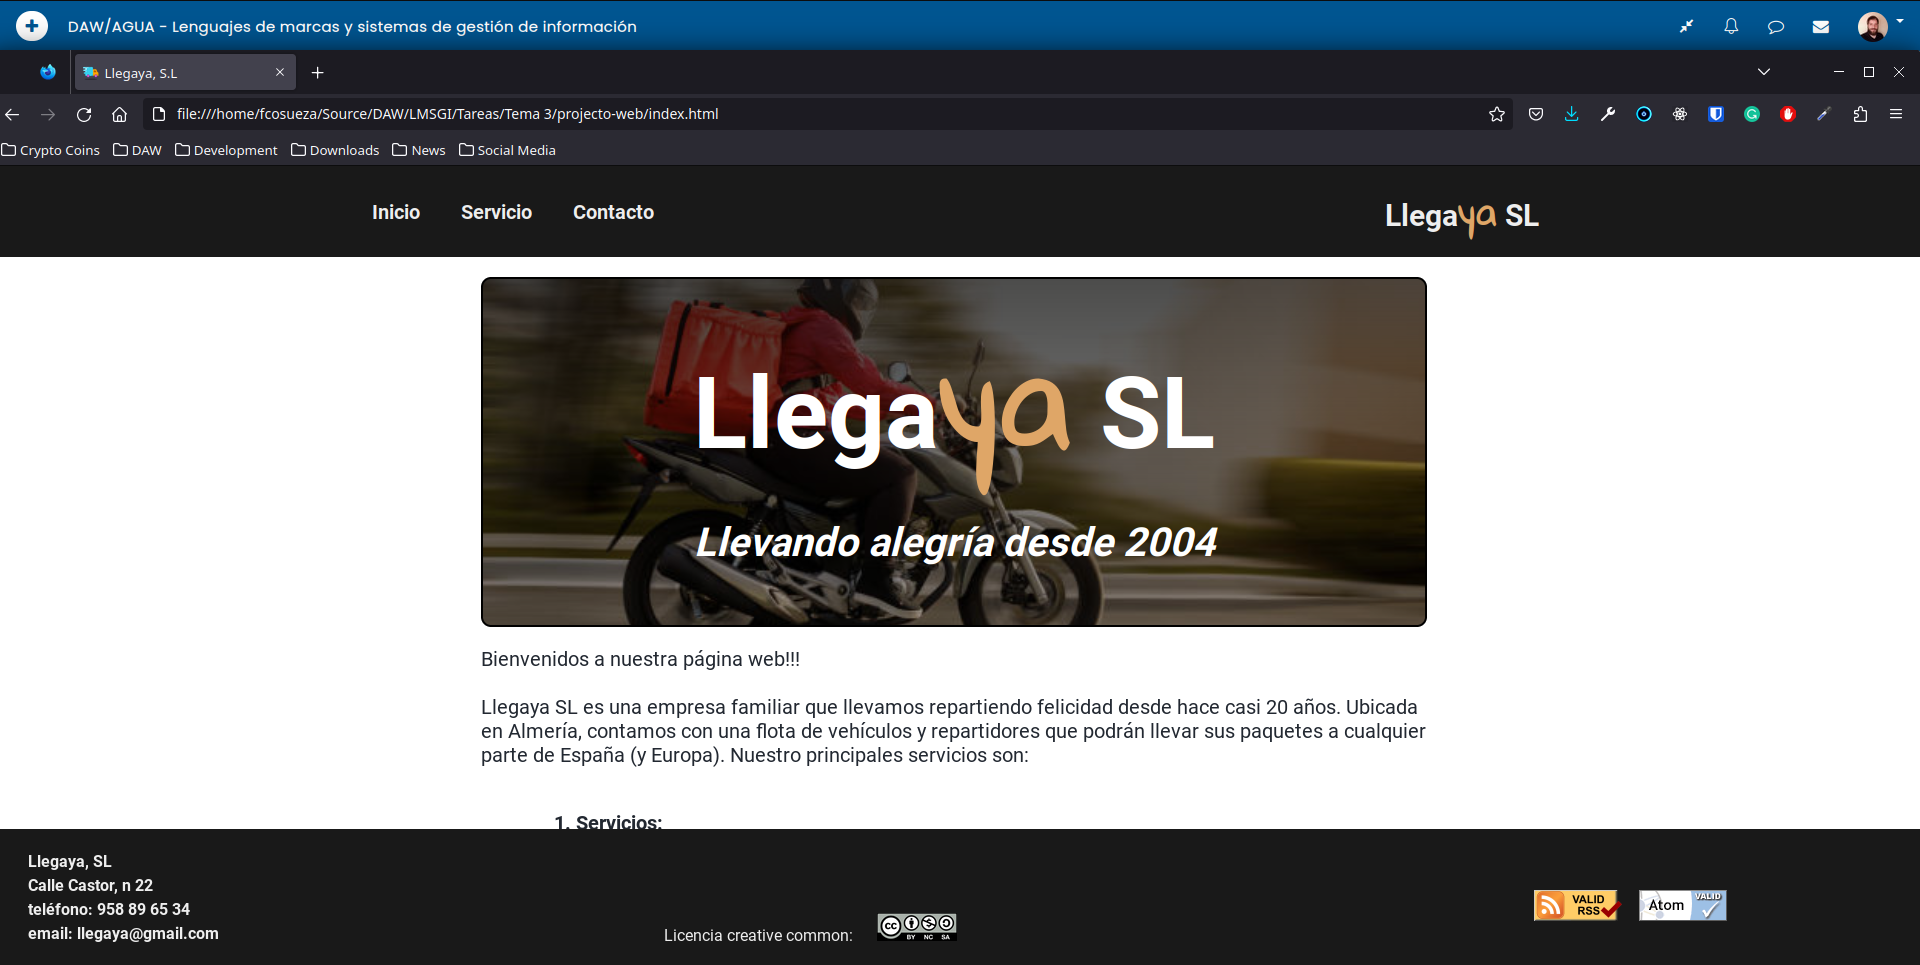
\includegraphics[scale=0.30]{channels-web.png}
    \caption{Página Web con los canales añadidos en el pie de página}
\end{figure}

\subsection{Solución Apartado D: Usando Thunderbird como Agregador de Noticias}
En este apartado vamos a usar un agregador de feeds para agregar un canal y consultar algunas de sus noticias. En nuestro caso, vamos a usar \textbf{Thunderbird}, ya que es el gestor de correo que estamos usando. Para ello, hemos seguido los siguientes pasos:

\begin{enumerate}
    \item Nosotros no hemos necesitado \textbf{descargar e instalar Thunderbird}, ya que es el gestor de correo que viene por defecto en Kubuntu y el que suelo usar. Pero si no fuera el caso, abría que descargar Thunderbird desde su \href{https://www.thunderbird.net/es-ES/}{página oficial}, siguiendo las instrucciones de instalación según el sistema operativo donde queramos instalarlo.

    \item Una vez instalado, deberemos \textbf{crear una cuenta de feeds}. En nuestro ya teníamos una creada, pero si no fuera el caso, podemos crear una pulsando en la opción del menu \textbf{File -> New -> Feed Account...}, que nos mostrará una ventana que nos guiará por el proceso de creación de la cuenta, como podemos ver en la siguiente captura.

    \begin{figure}[H]
        \centering
        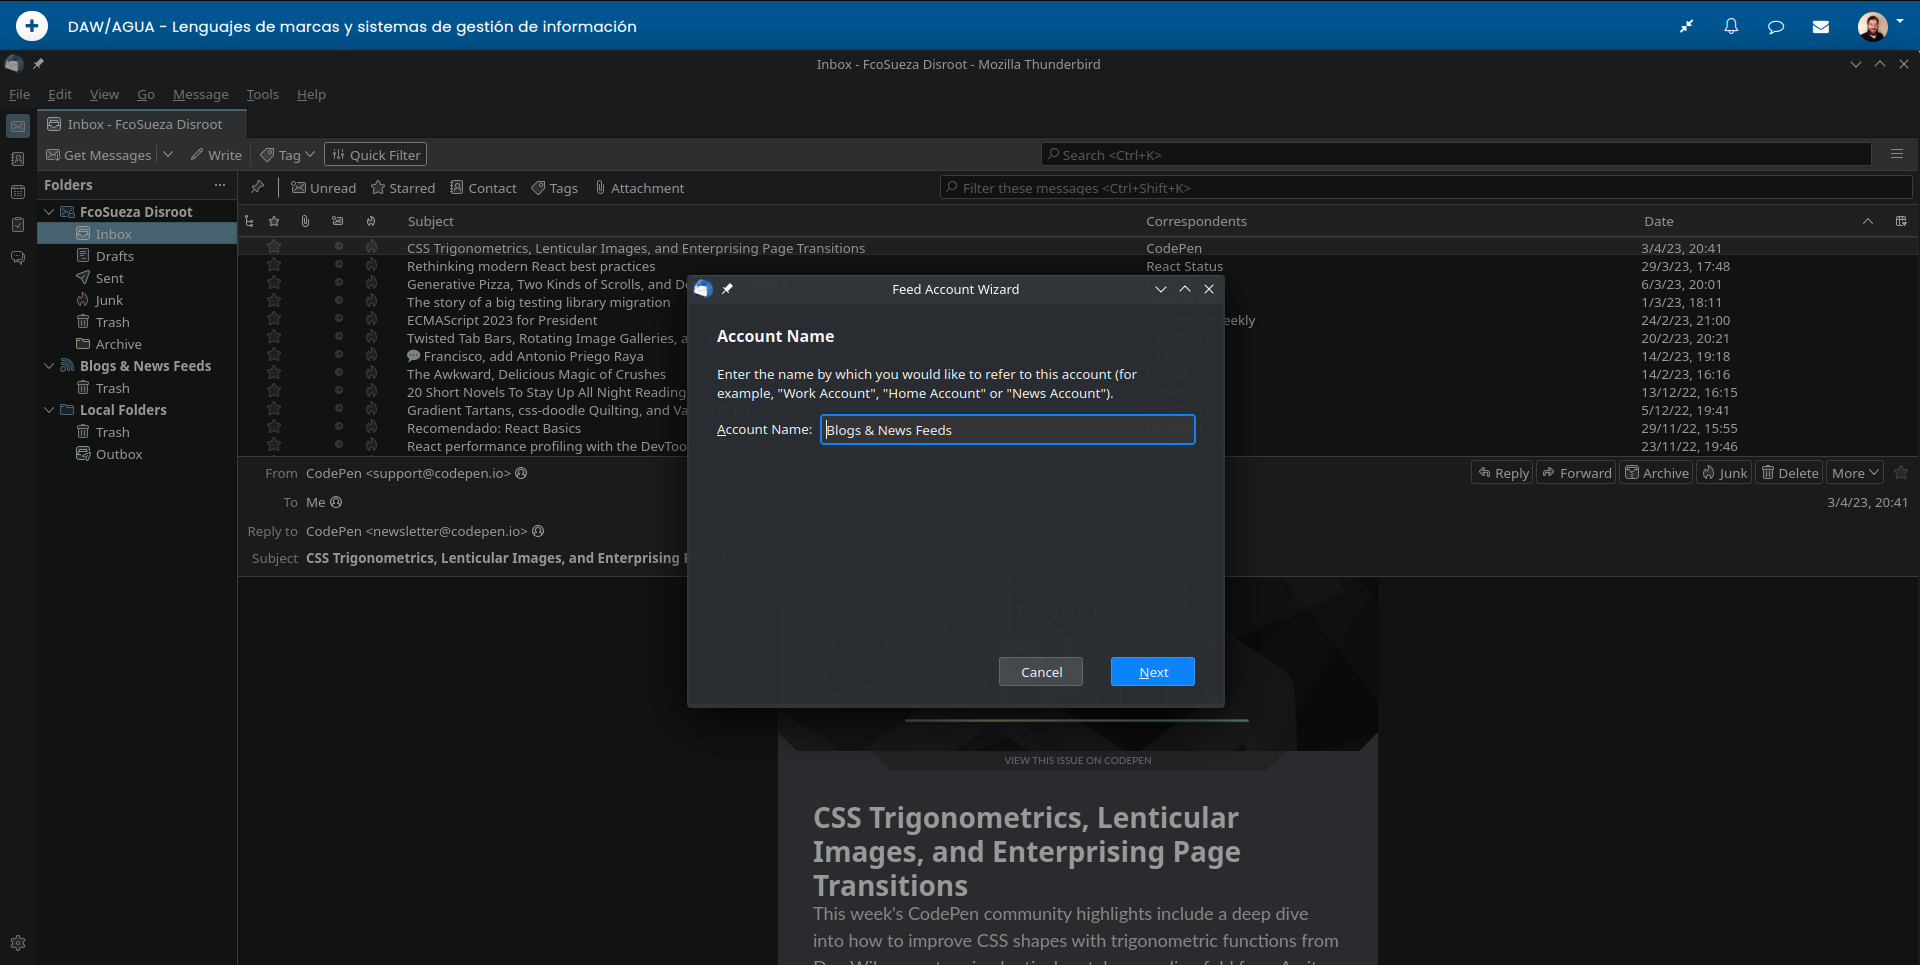
\includegraphics[scale=0.27]{thunderbird-1.png}
        \caption{Creación de la cuenta de feeds en Thunderbird}
    \end{figure}

    \item Lo siguiente ha sido buscar un canal de noticias de alguna empresa de paquetería. En nuestro caso ha sido complicado encontrar un canal de una empresa nacional, por lo que hemos buscado en empresa extranjeras donde teníamos varias opciones, pero al final, nos hemos decidido por \textbf{FedEx}. En concreto, en su división  \href{https://fedexbusinessinsights.com/}{FedEX Bussines Insight},

    Así, usaremos la dirección \url{https://fedexbusinessinsights.com/feed/} para añadir a Thunderbird y suscribirnos al canal RSS de FedEx.

    \item Para añadir el canal RSS a Thunderbird solo tenemos que pulsar con el botón derecho sobre el canal que de Feeds que se habrá creado y que se mostrará en el menú desplegable que se encuentra a la izquierda de la interfaz de Thunderbird, como podemos ver en la siguiente imagen, y pulsar en la opción \textbf{Subscribe}.

    \begin{figure}[H]
        \centering
        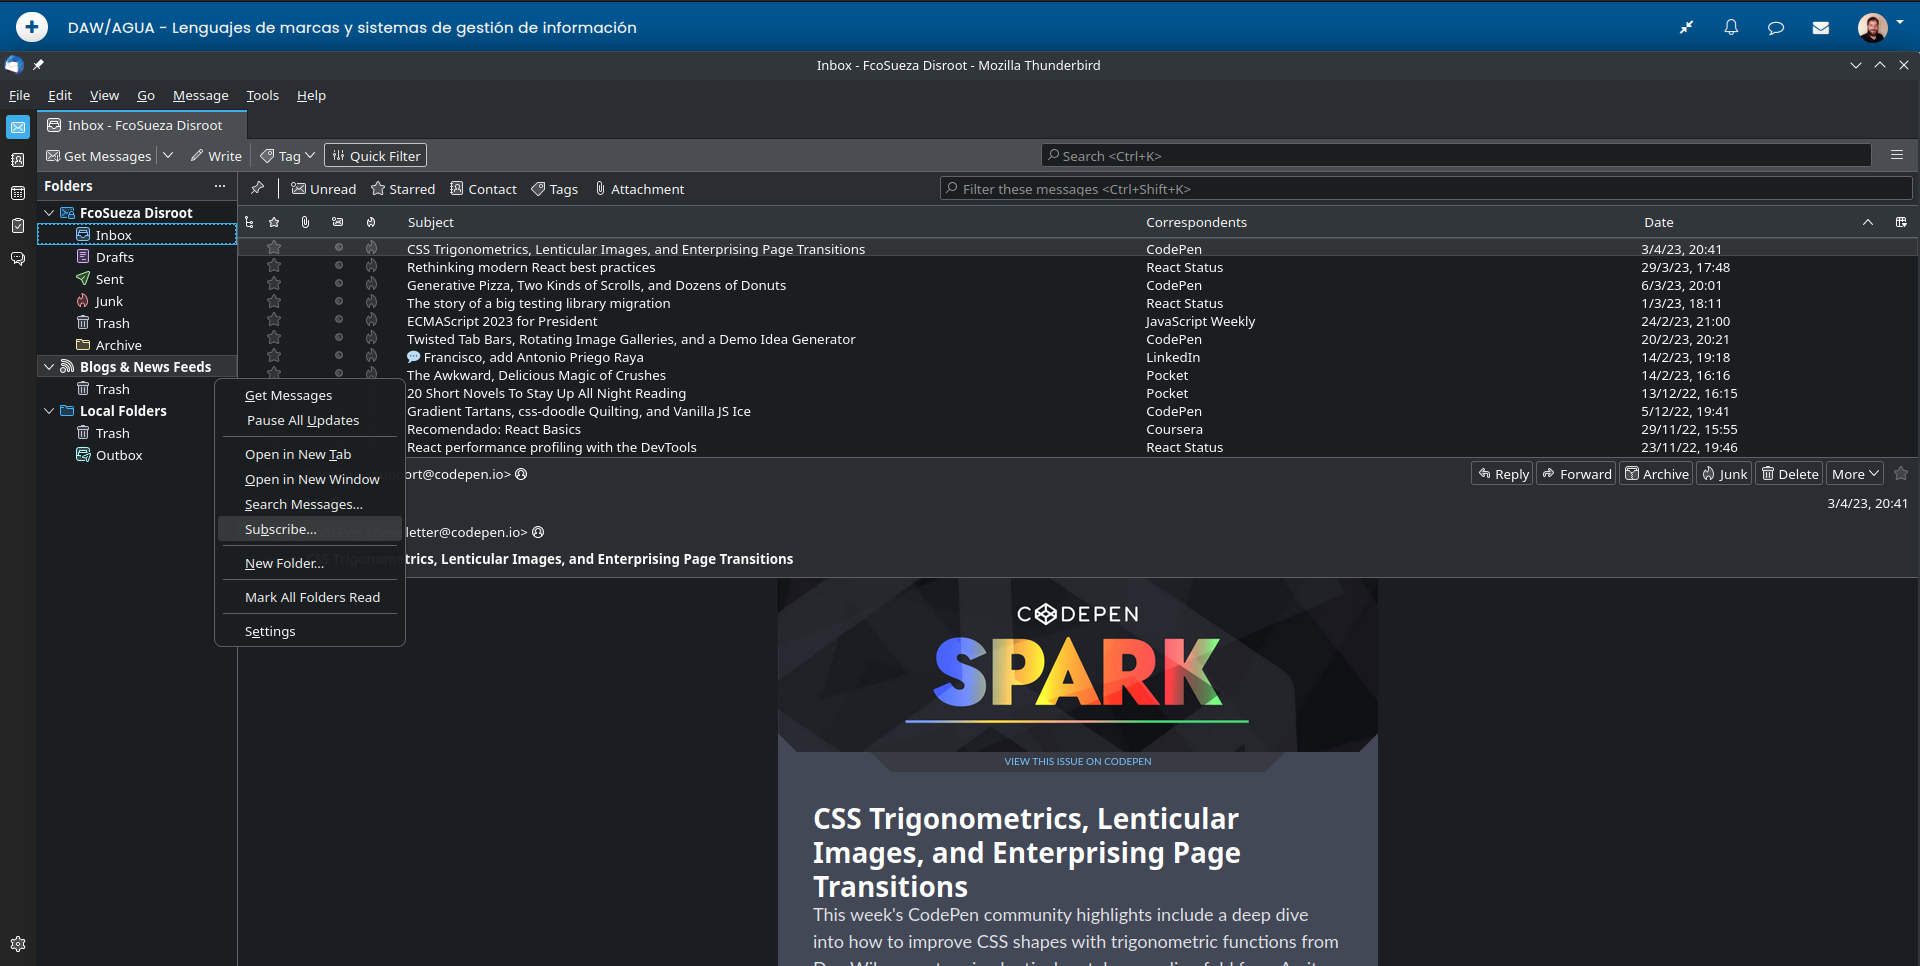
\includegraphics[scale=0.27]{thunderbird-2.png}
        \caption{Añadiendo el feed a Thunderbird}
    \end{figure}

    En la ventana que se nos abrirá, debemos introducir la URL que hemos comentado arriba y pulsar en el botón \textbf{add}. Si todo va bien, se nos mostrará una ventana con los datos del canal de noticias. Si pulsamos en \textbf{Verify}, se verificará el canal y se añadirá a Thunderbird.

    \begin{figure}[H]
        \centering
        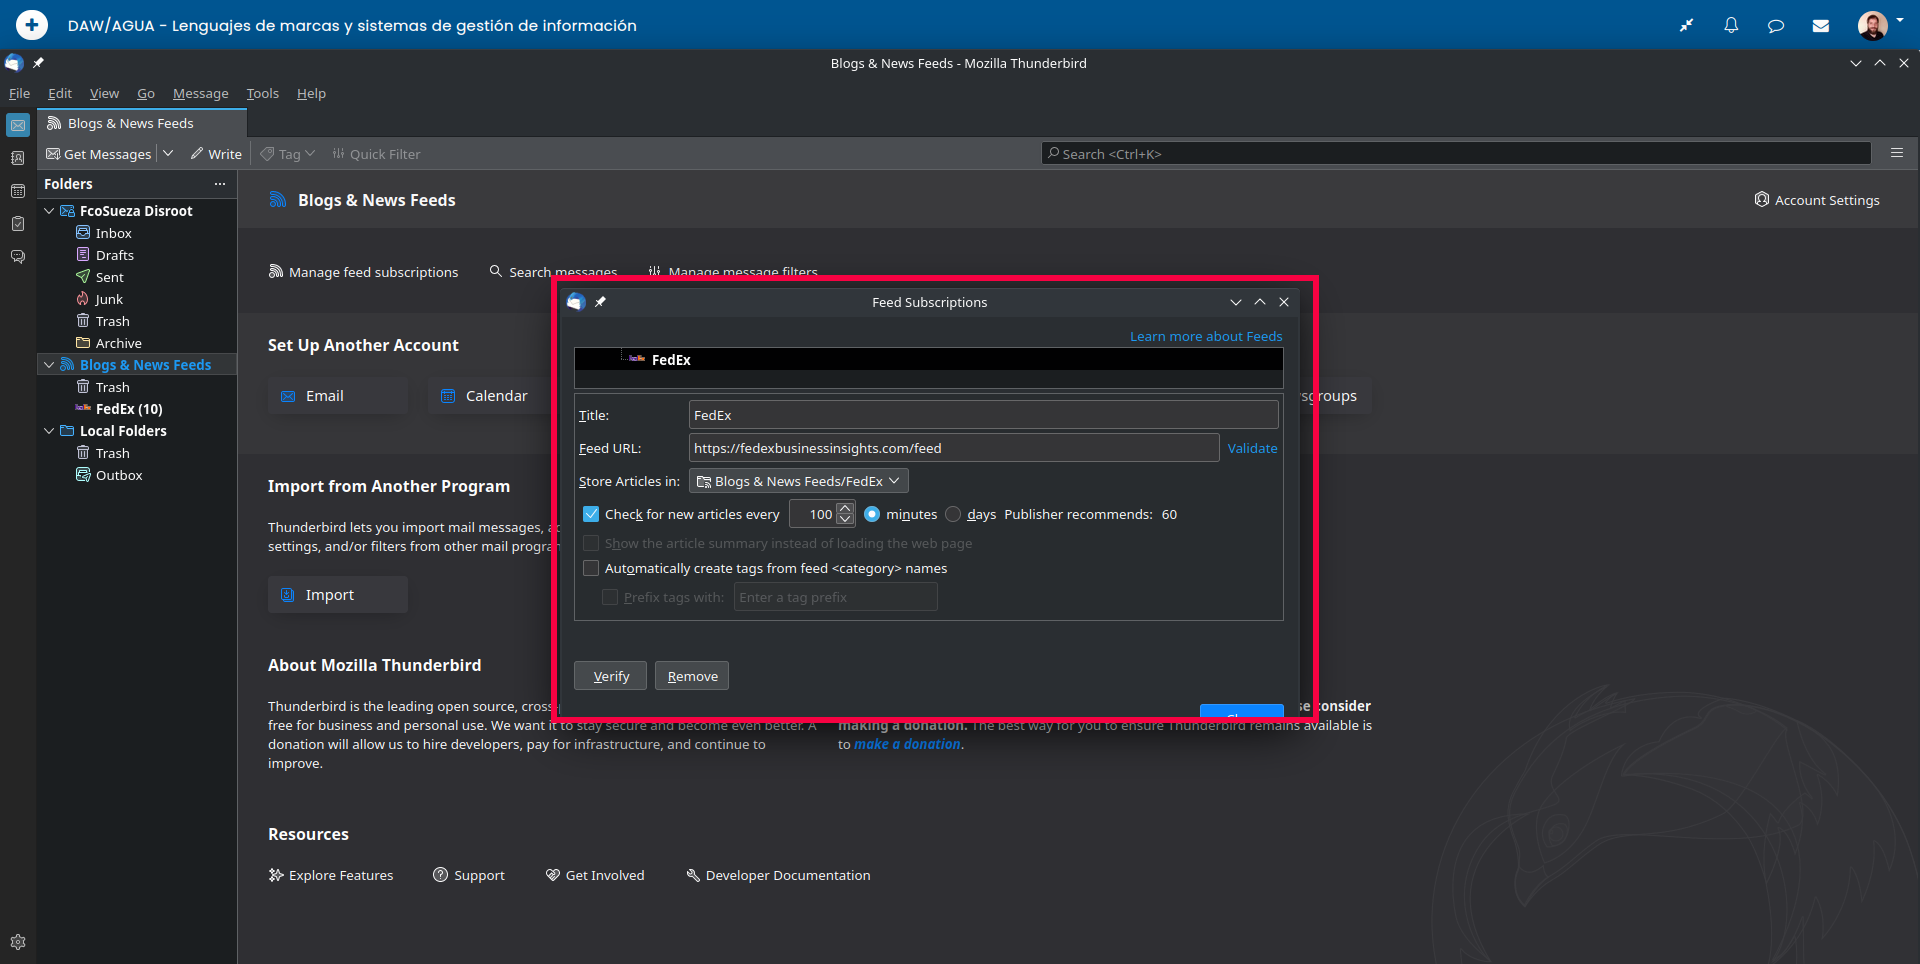
\includegraphics[scale=0.27]{thunderbird-3.png}
        \caption{Ventana verificación canal de noticias en Thnderbird}
    \end{figure}

    \item Una vez realizado esto, tendremos añadido el canal de noticias y podremos acceder a ellas como si fuera una cuenta de correo. En la siguiente imagen podemos ver, resaltados con una cuadrado en rojo, tanto el canal ya añadido en la sección de feeds como la lista de noticias de dicho canal.

    \begin{figure}[H]
        \centering
        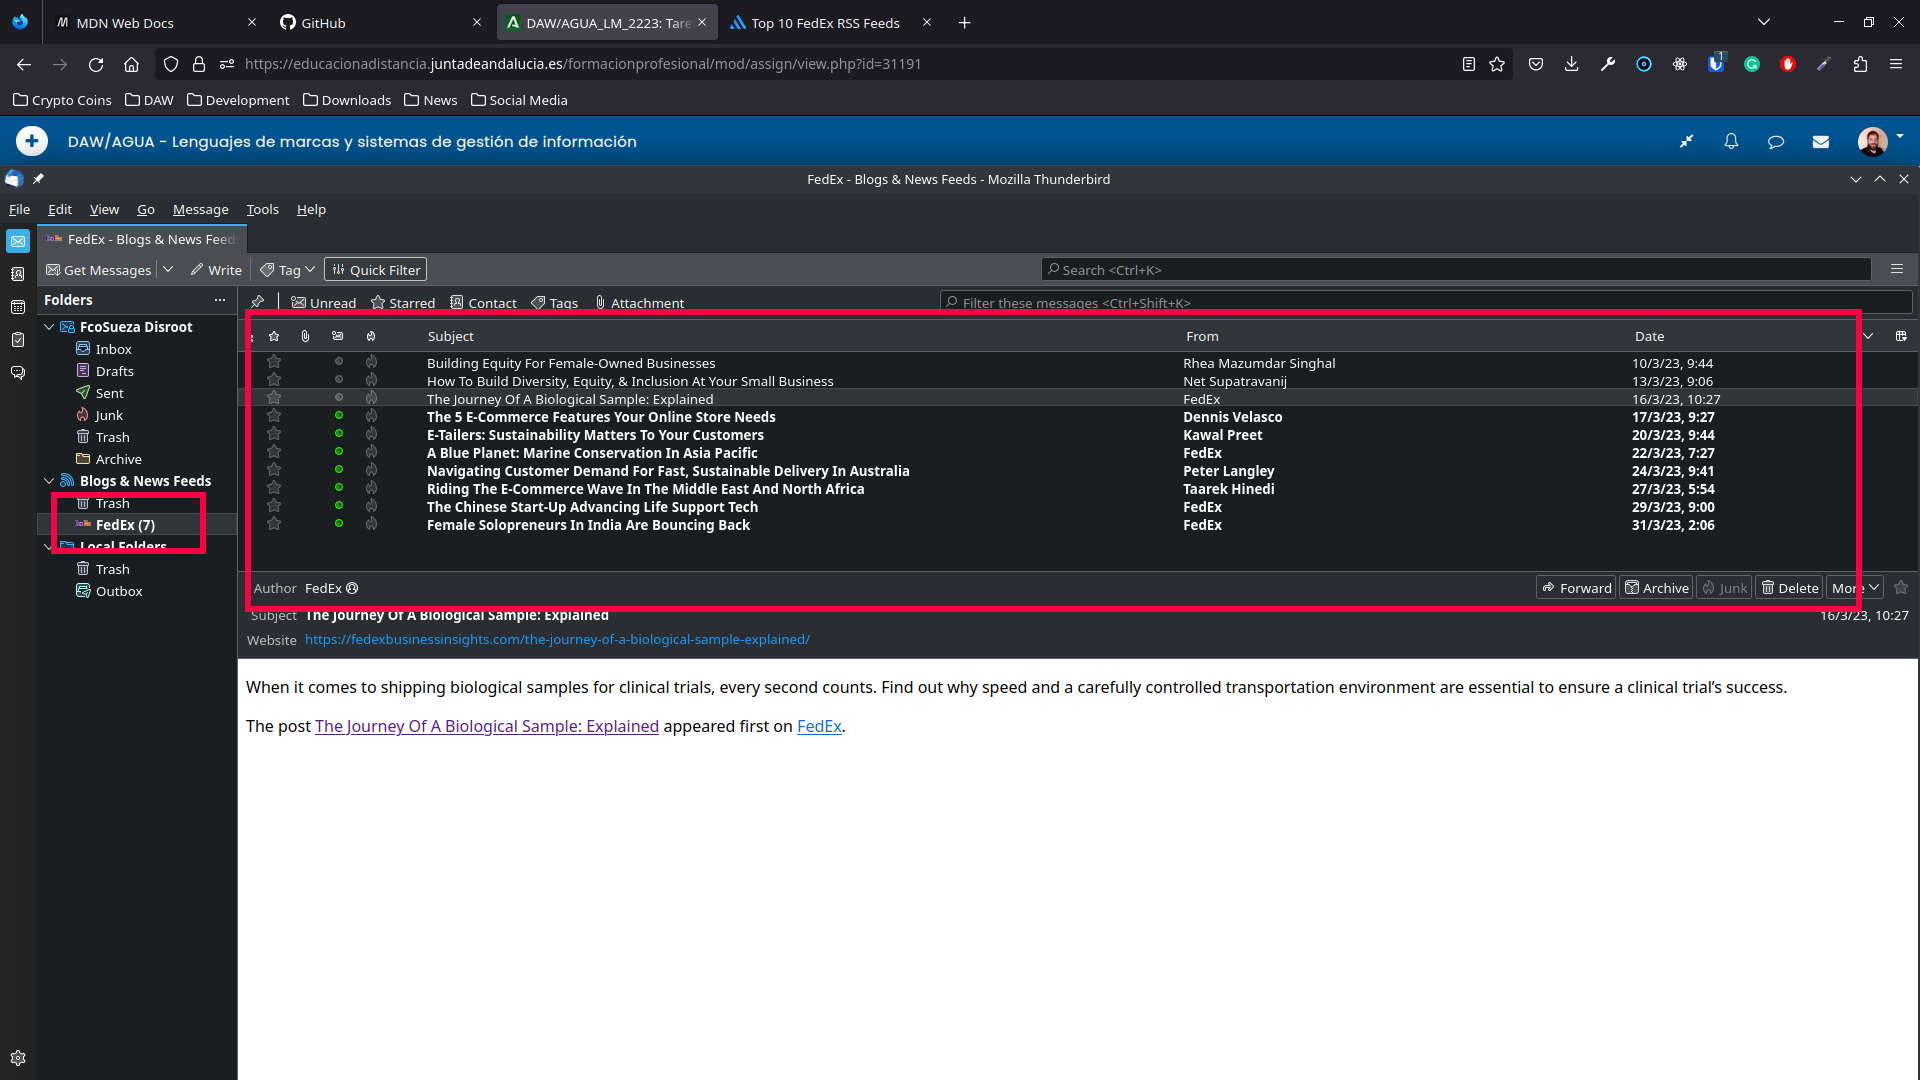
\includegraphics[scale=0.27]{thunderbird-4.png}
        \caption{Canal de noticias añadido y lista de noticias}
    \end{figure}
\end{enumerate}

% Bibliography

%\newpage

%\bibliography{citas}
%\bibliographystyle{unsrt}

\end{document}